\chapter{Objetivos e características}

Os objetivos do gerenciamento do escopo do projeto são: definir o que está e o que não está incluso no projeto e assegurar que o projeto inclui todo o trabalho necessário, e \textbf{apenas o necessário}, para terminar o projeto com sucesso.

Os processos que fazem parte do gerenciamento do escopo, representados na Figura \ref{fig:proc:ger:escopo}, podem ser resumidos em:

\begin{itemize}
	
	\item[\textbf{Coletar os requisitos}]: definir e documentar as necessidades das partes interessadas para alcançar os objetivos do projeto.
	
	\item[\textbf{Definir o escopo}]: desenvolver uma descrição detalhada do projeto e do produto.
	
	\item[\textbf{Criar a EAP}]: subdividir as entregas e o trabalho do projeto em componentes menores e mais facilmente gerenciáveis.
	
	\item[\textbf{Verificar o escopo}]: formalizar a aceitação das entregas terminadas do projeto.
	
	\item[\textbf{Controlar o escopo}]: monitorar o progresso do escopo do projeto e escopo do produto e gerenciar as mudanças feitas na linha de base do escopo.	

\end{itemize}

\begin{figure}[!h]
	\centering
	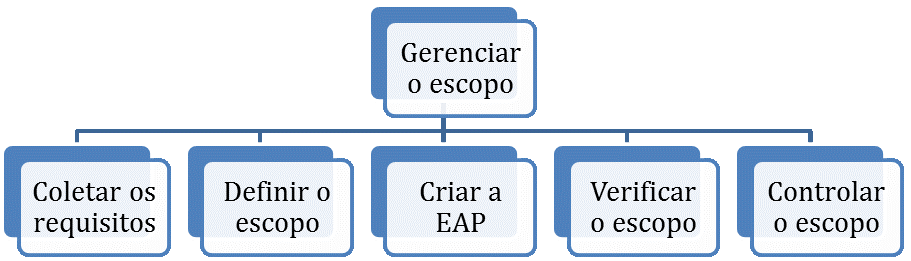
\includegraphics[scale=0.75]{Figuras/gerenciamento_escopo.png}
	\caption{Processos do Gerenciamento do escopo}
	\label{fig:proc:ger:escopo}
\end{figure}

\section{O que é escopo}


Esse é o \textbf{Escopo do projeto} que não deve ser confundido com o \textbf{Escopo do produto}, que são os atributos, funcionalidades e características que devem estar presentes no produto ou serviço criado pelo projeto, conforme podemos observar na Figura \ref{fig:escopo:proj:prod}.

\begin{figure}[!h]
\centering
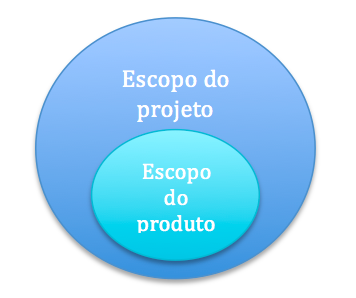
\includegraphics[scale=0.5]{Figuras/escopo_proj_prod.png}
\caption{Escopo produto X escopo projeto}
\label{fig:escopo:proj:prod}
\end{figure}

\section{Gerenciamento do Escopo}

Sãos os processos que visam garantir que o projeto inclua todo o trabalho necessários para completar com sucesso o projeto.

Para isso, deve incluir:

\begin{itemize}

\item Definir e controlar o que \textbf{faz} e o que \textbf{não faz} parte do projeto.

\item Controlar se todo o trabalho está sendo realizado.

\item Controlar o processo de mudanças do escopo.

\item Confrontar as mudanças com o \termo.

\item Evitar retrabalho ou trabalho desnecessário e seus custos

\end{itemize}

\section{Processos}

Para garantir a gerência do escopo, são necessários os seguintes processos:

\begin{itemize}

\item \textbf{Coleta de requisitos}: definir e documentar o que é necessário para se alcançar os objetivos do projeto.

\item \textbf{Definição do escopo}: descrição detalhada do projeto e do produto.

\item \textbf{Criação da Estrutura Analítica do Projeto (EAP)}: a fim de facilitar o gerenciamento das entregas e do trabalho, o escopo deve ser dividido em partes menores e estruturadas.

\item \textbf{Verificação do escopo}: formalizar a aceitação das entregas finalizadas do projeto.

\item \textbf{Controle do escopo}: monitorar e gerenciar o andamento e as mudanças na linha de base do escopo.

\end{itemize}

Os processos dentro do ciclo de vida do projeto podem ser observados na Figura \ref{fig:ciclo:vida}.

\begin{figure}[!h]
\centering
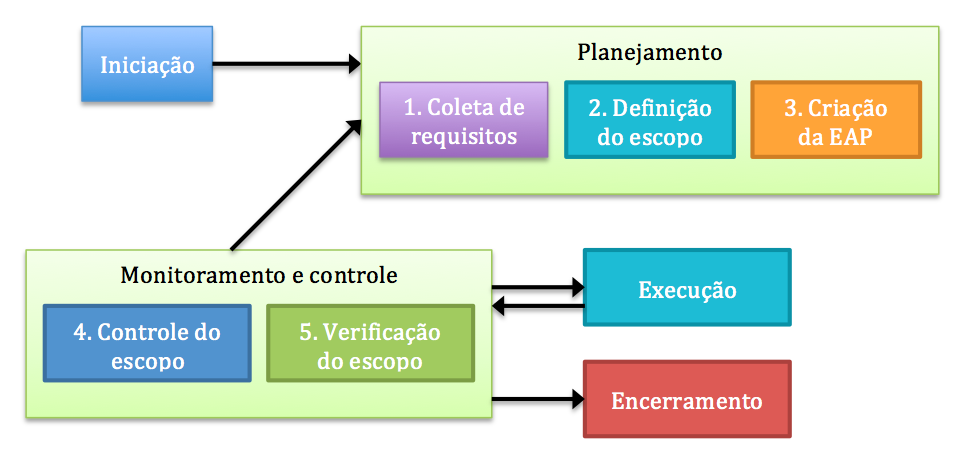
\includegraphics[scale=0.5]{Figuras/ciclo_vida.png}
\caption{Processos dentro do ciclo de vida do projeto}
\label{fig:ciclo:vida}
\end{figure}

\subsection{Inimigos do escopo}

Um escopo com problemas pode levar o projeto ao seu fim. Por isso é importante observar os dois principais inimigos do escopo:

\begin{itemize}

\item \textbf{\textit{Scope Creep}}: aumento do escopo sem nenhum controle, de maneira contínua, muitas vezes de forma lenta, que resulta em um escopo ``inchado'', ingerenciável, cujo foco foge da ideia inicial do projeto e o resultado reflete no aumento dos custos e perda de prazos.

\item \textbf{\textit{Gold Plating}}: adicionar elementos não especificados nos requisitos do projeto, geralmente partindo de equipes técnicas e de desenvolvimento sob a alegação de agregar valor mas cujo resultado é o aumento de custos, perda de qualidade e aumento desnecessário da complexidade do produto.

\end{itemize}

\subsection{Requisitos}

São condições ou capacidades que devem ser supridas pelo resultado do projeto (produto ou serviço) a fim de satisfazer um contrato ou outro documento formal.

São dividos em:

\begin{itemize}

\item \textbf{Requisitos funcionais:} o que o produto ou serviço deve \textbf{fazer}.

\item \textbf{Requisitos não-funcionais:} o que o produto ou serviço deve \textbf{ter}.

\end{itemize}